% Emacs, this is -*-latex-*-

\title{Information Theory}
\maketitle

\tableofcontents

\section{Rate}

In a communication system, the
\href{https://en.wikipedia.org/wiki/Bit_rate}{rate} describes the
amount of data (for example, bits) that is transmited by time unit
(for example, a second). Such rate depends on:
\begin{enumerate}
\item The
  \href{https://en.wikipedia.org/wiki/Entropy_(information_theory)}{entropy}
  of the information represented by the data. The higher the entropy,
  the higher the rate.
\item The encoding scheme (usualy known as the
  \href{https://en.wikipedia.org/wiki/Entropy_coding}{entropy coding})
  using for representing the information.
\end{enumerate}

\section{Distortion}

In an lossy encoding system, the distortion (expressed for example by
the \href{https://en.wikipedia.org/wiki/Mean_squared_error}{MSE})
measures the amount of error between two signals: the original signal
and the distorted one. The origin of this error can be quite varied
and ranges from transmission errors to quantization processes.

\section{The RD (Rate/Distortion) curve}

A RD curve represents the distortion versus the rate (i.e, the
\href{https://en.wikipedia.org/wiki/Rate-distortion_theory}{RD
  performance}) of any lossy encoding system. Basically, a RD curve
express the compresibility of different approximations to the
information generated by a source of data.


For example, when the signal is quantized, rate and distortion are
``opposed'' features of the encoding system in the sense that, for
example, if the bit-rate is descreased, the distortion is increased,
and viceversa. Such variables (Rate (R) and Distortion (D)) can be
represented as a curve.

such as the shown in the
Fig.~\ref{fig:RD_slopes}.

Usually, RD curves are convex, which means
that if $\lambda_i$ is the slope of the curve measured at the $i$-th
point of the curve (starting at the lowest bit-rate), it usually hold
that
\begin{equation}
  \lambda_i > \lambda_{i+1}.
  \label{eq:convexity}
\end{equation}
where $\lambda$ quantifies the trade-off between decreasing the
distortion\footnote{For this reason, the slopes are negative.} while
the bit-rate
increases~\cite{vetterli1995wavelets,sayood2017introduction}. However,
Eq.~\eqref{eq:convexity} is not always true in the real world.

Notice that, the higher the slope, the higher the benefit in terms of RD.

%}}}

\section{RDO (Rate/Distortion) Optimization}

\begin{figure}
  \centering
  %\svgfig{graphics/RD_slopes}{8cm}{800}
  %\svg{graphics/RD_slopes}{800}
  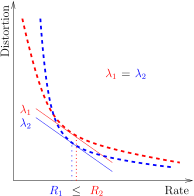
\includegraphics[width=1.0\textwidth]{graphics/RD_slopes} 
  \caption{Two RD (Rate/Distortion) curves.}
  \label{fig:RD_slopes}
\end{figure}

RDO is a process that arises when we need to encode at the same time
two or more different sources of data, $A$ and $B$. When this happens,
each source has own charateristic RD curve (see the
Fig.~\cite{RD_slopes}).

If we suppose now that the contribution to the distortion of the
quantization of each source is independent\footnote{The distortion
generated in one of the sources does not influence the distortion
generated in the other source.} and additive\footnote{Or in general, a
linear combination of the distortions, where each source contributes
more than the other(s) to the total distortion $D$.}, that is
\begin{equation}
  D = D^A + D^B,
  \label{eq:additive}
\end{equation}
where $D$ denotes distortion, then the optimal quantization steps must
satisfy that~\cite{vetterli1995wavelets,sayood2017introduction}
\begin{equation}
  \lambda^A_i = \lambda^B_i.
  \label{eq:optimal_quantization}
\end{equation}

To see this, lets suppose that we have used, for example, a set of
quantization step sizes so that $\lambda^A_i/2 = \lambda^B_i,$ and
that we still have room for more bits to encode the frame. In this
situation, the maximum benefit would be obtained if and only if we
decrease $\Delta^A_i$ (modifiying the corresponding
$\mathbf{\Delta}_i$), because the slope for the source $A$ doubles
the slope of the source $B$. Therefore, the optimal quantization
steps are obtained when Eq.~\ref{eq:optimal_quantization} is
true.


\section{Resources}
%{{{ 
\renewcommand{\addcontentsline}[3]{}% Remove functionality of \addcontentsline
\bibliography{data-compression,signal-processing,DWT}
%}}}
